% \documentclass[a4paper,10pt]{article}
 \documentclass[review]{myarticle}
\usepackage[utf8]{inputenc}

\usepackage{graphicx}
\usepackage{graphics}
\usepackage{enumitem}

\usepackage{epsfig}
\usepackage{subfigure}
\usepackage{tabularx}
\usepackage{amssymb}
\usepackage{amsmath}

\usepackage{enumitem}
\usepackage{a4wide} %full page
\usepackage{hyperref}
\usepackage{natbib}
\usepackage{amsmath,amssymb}
\usepackage{setspace}
\usepackage[scientific-notation=true]{siunitx} %VVV
\sisetup{round-mode = places, round-precision = 3} %VVV
\doublespacing

\usepackage{booktabs}
\usepackage{multirow}
\usepackage{url}

 \RequirePackage{lineno} 

\bibliographystyle{model2-names}
\biboptions{authoryear}

\newenvironment{lineq}
    {\begin{linenomath*}
    \begin{equation}
    }
    { 
    \end{equation} 
    \end{linenomath*}
    }


\newcommand{\dd}{\mathrm{d}}
\renewcommand{\vec}{\mathbf}
 \newcommand{\subscript}[2]{$#1 _ #2$}

 \newcommand{\Lb}{\pazocal{L}}
 


%opening

\usepackage[table]{xcolor} 

\begin{document}

\begin{frontmatter}

\title{Issues in the inverse modeling of a soil infiltration process}

\author[autor1]{Michal Kuraz}

\author[autor1]{Lukas Jacka}

\author[autor2]{Matej Leps}

\author[autor1]{Vojta Havlicek}

\address[autor1]{Czech University of Life Sciences Prague, Faculty of Environmental Sciences, Department of Water Resources and Environmental Modeling}

\address[autor2]{Czech Technical University in Prague, Faculty of Civil Engineering, Department of Mechanics}

\begin{abstract}
This contribution addresses issues in evaluation of the soil hydraulic parameters (SHP) from the Richards equation based inverse model. The inverse model was representing single ring infiltration experiment on mountainous podzolic soil profile, and was searching for the SHP parameters of the top soil layer. Since the thickness of the top soil layer is often much lower than the depth required to embed the single ring or Guelph permeameter device, the SHPs for the top soil layer are very difficult to measure directly. The SHPs for the top soil layer were therefore identified here by inverse modeling of the single ring infiltration process, where, especially, the initial unsteady part of the experiment is expected to provide very useful data for evaluating the retention curve parameters (excluding the residual water content) and the saturated hydraulic conductivity. 

The main issue, which is addressed in this contribution, is the uniqueness of the Richards equation inverse model. We tried to answer the question whether is it possible to characterize the unsteady infiltration experiment with a unique set of SHPs values, and whether are all SHP parameters vulnerable with the non-uniqueness. Which is an important issue, since we could further conclude whether the popular gradient methods are appropriate here. Further the issues in assigning the initial and boundary condition setup, the influence of spatial and temporal discretization on the values of the identified SHPs, and the convergence issues with the Richards equation nonlinear operator during automatic calibration procedure are also mentioned here.
\end{abstract}

\begin{keyword}
soil hydraulic parameters \sep inverse modeling of Richards equation \sep influence of spatial and temporal discretization on  solution of the Richards equation \sep application of dd-adaptivity algorithm \sep computational hydrology

%% MSC codes here, in the form: \MSC code \sep code
%% or \MSC[2008] code \sep code (2000 is the default)

\end{keyword}

\end{frontmatter}

\linenumbers

\section{Introduction}%[lukas]
% -motivace

Soil hydraulic parameters (SHP), mainly saturated hydraulic conductivity and the parameters of the retention curve, are important for many hydrological models and engineering applications.  The mountainous podzolic soil evaluated here is typical for the source areas of many major rivers in the Central European region. The top layer of the soil plays a key role in the rainfall-runoff process, because it is the top-soil that separates the rainfall into surface runoff and subsurface runoff. The top-soil layers, especially in the case of a mountain forest soil, exhibit large temporal and spatial changes in soil structure (and therefore large variability in SHPs), mainly due to seasonal changes in vegetation activity, changes in root density and root volume, irregular distribution of various plant species on the soil surface, and a distinct alternation of wetting and drying cycles \citep{Fodor,Schwen, Leij, Mubarak}.



Due to the rocks that are present and the dense root system of the covering vegetation, and due to the possible extension of the representative elementary volume, it is often impossible to collect undisturbed samples of top-soil for laboratory measurements in order to obtain the saturated hydraulic conductivity and the parameters of the retention curve~\citep{Jacka1}. The SHPs of the top-soil are therefore very difficult to measure directly~\citep{Fodor, Jacka1}. 


In our study, the well-known single ring method (SR) was used to obtain experimental input data (cumulative infiltration) for inverse modeling. The  single ring infiltrometer (SR) is a widely accepted, simple, robust field method, which is able to measure infiltration process, which affects the entire soil profile including the top-soil,  and can sample a relatively large volume (depending on the diameter of the ring)~\citep{Cheng,ReynoldsWD}.  The single ring (SR) infiltration experiment is an in situ experiment, which does not require soil samples to be collected, so the porous media is naturally undisturbed. With the widely-used ring diameter of 30~cm, the affected porous media is far more representative than any soil sample  we were able to collect. However, the top-soil can also be measured (with some alteration of the surface) using other well-known field infiltration methods, e.g. the tension infiltrometer or the well permeameter (see \citep{AnguloJaramillo,ReynoldsWDGP}). 
 It should be mentioned here that the ring  infiltration exhibits some of the following issues: 1) air may be entrapped in some pores during rapid flooding of the soil surface inside the ring, 2) the flow geometry and the  initial conditions are not known exactly for the entire profile and 3) the boundary conditions (with the exception of the surface of the ring) are difficult to estimate  \citep{Jacka1,Fodor}.
Since the flow in a variably saturated porous medium is governed by the Richards equation, where the soil properties are described by SHPs, it is expected that the Richards equation can be used for inverse analysis of the of SHPs the top-soil on the basis of the measured infiltration data. It is apparent that the both unknown saturated and residual water content yield non-unique solution of Richards equation inverse model, the residual water content should be excluded from the identification.

Over the last three decades the Richards equation became challenging topic for many proprietary and opensource projects. 
 One of the most well-known code from the proprietary group is Hydrus~\citep{SimunekJ} and FEFLOW~\citep{feflow}. From the opensource group there has recently formed a large community around the project Open Porous Media~\citep{opm} which includes also the well-known DuMu$^{\textrm{X}}$~\citep{dumux} project. However, in this contribution we made use of another opensource project DRUtES~\citep{drutes}, which includes features for efficient solutions of problems with progressive breakthrough (such as the moving wetting front) based on domain decomposition techniques, for details see~\citep{mojecomp, mojejcam2, mojeamc2}.


 Several studies have compared inverse modeling and tension infiltrometers (see e.g. \citep{Verbist, Simunek1, Ventrella, Schwartz, Ramos, Simunek2}). It states that the retention curves obtained from the inverse modeling of the Richards equation using tension infiltrometer data are often not in good agreement with laboratory experiments on undisturbed samples (see e.g. \citep{rezaei}). In particular, the saturated water content obtained from an inverse model based on  the Richards equation is typically distinctly lower than the experimentally established value (see e.g.~\citep{Simunek1, Verbist}). This could be due to the following effects: the effect of hysteresis as a drying process in the laboratory differs from the wetting process in the field; the effect of entrapped air in the field (see e.g.~\citep{Fodor}), where the saturation may not fully correspond the pressure head, and an effect of macropores, which are excluded when a tension infiltrometer is used. An most importantly the soil samples, which are usually  examined in the laboratory, are typically much smaller than the representative elementary volume~\citep{scharnagl}.
 However, it should be mentioned here that a few studies have reported a close correspondence between the retention curve parameters obtained from laboratory experiments and from the Richards equation based inverse model (see e.g.\citep{Ramos} or~\citep{Schwartz}).

The non-uniqueness of the Richards equation based inverse model was studied by \citep{beven2003-uncertain}. It was demonstrated on real world case study of Sherwood Sandstone Aquifer that many different SHP parameters of macroscopic media representing the layered  unsaturated zone provided acceptable simulations of the observed aquifer recharges. However, in this work 
the non-unique definition with the unknown residual and saturated water content was considered.
The definition of unique inverse function for identification of macroscopic media was treated in~\citep{zou200126}, where the recommended approach was to assemble the objective function from transient data of the capillary pressure and from the steady state water content data. Another issue is the equifinality in the mathematical model setup in terms of the initial and boundary condition data, this problem was studied by~\citep{klaus-hydrol}.

And yet another challenging issue is the treatment of the nonlinear operator of the Richards equation. \cite{beven2003-uncertain} reported that during his Monte Carlo simulations on wide ranges of SHPs values 56\% of simulations were rejected, because of convergence problems. 
Despite it wasn't mentioned in the paper explicitly, we can suggest that these convergence issues originated from the nonlinear operator treatment -- the outer iterations.
It could be easily concluded, that if we use simple Picard method for the nonlinear operator, and we increase the iteration criterion, we will obtain less accurate solution but we will also require less iterations for the Picard method. If we further increase the criterion we will end up with semi-implicit solution, where the constitutive functions in the Richards equation are evaluated from the previous time level solution -- thus we will always need just a single outer iteration.



And so the following questions arise. 
\begin{itemize}
\item Is it possible to approximate our relatively simple inverse Richards equation problem, where the only unknown parameters represent the thin top-soil layer, by a unique set of SHPs (excluding the residual water content, which was neglected -- assumed to be zero)?
\item If not are all SHPs parameters vulnarable with this non-uniqueness?
\item Is it acceptable to use here the popular gradient methods to obtain these parameters, since the gradient methods have been very popular since 1980s, see~\citep{vangen-old}, until recent, see e.g.~\citep{rezaei, Verbist2010, Ventrella, Simunek2}?
\item How much are SHP parameters identified by inverse analyses of SR infiltration dependent on the treatment of the nonlinear operator of the Richards equation? Is there any benefit in using the accurate Newton or Picard iteration method, or can we obtain a reasonable estimate with just the semi-implicit solution (all constitutive function values are obtained from the previous time level solution)?
\end{itemize}



The aim of this paper is to answer these proposed issues. The inverse modeling problem applied here for evaluating these issues will not be a synthetic case but will be a real world problem of identification of the SHP parameters for top soil podzolic horizons of experimental catchment Modrava, Sumava National Park, Czech Republic.  The SHPs for the lower horizons were already identified by various laboratory experiments and by data processing (e.g. pedotransfer functions, see Rosetta code~\citep{Schaap}), only the top soil SHPs are difficult to  obtain directly. Moreover, for this type of top soil layer it is even a very difficult to guess some limited ranges of its SHPs. However, the knowledge of the lower horizons should limit the non-uniqueness of this inverse problem. Apart answering the given questions, which are nearly classical but not satisfactory resolved issues in this field of research, we will also try to address issues with initial and boundary condition setup for the approximation of SR infiltration process. And finaly the numerical issues originating from the convection term in the Richards equation representing the axisymmetric SR infiltration flux will be also discussed in this work.









\section{Methodology}% [lukas a michal]
\label{metodo}

This section is divided into two distinct parts. The first part, section~\ref{assamb}, is focused on assembling the experimental data, which were later used for the inverse modeling. In this section the site description, the reconstruction of the parameters of the SHPs for the lower profiles, and the processing of the experimental data is given.   This section also provides a complete definition of the SHPs parameters -- the solution of our inverse problem -- particularly in the paragraph~\ref{shp}.

The second part of the methodology, section~\ref{invproc}, covers the main topic of this paper --  issues in the Richards equation based inverse model. The governing equation is given together with  notes about the numerical stability of the convection dominant problems, since it is not always mentioned that diffusion type equation in cylindric coordinates (such as the Richards equation or the groundwater flow equation) contains first order derivative term, which is a language of mathematics nothing else than a convection term, and so the numerical stability issues appear.
Further the issues in selecting an appropriate boundary conditions are discussed, since it is not easy to find an agreement between the mathematical model setup and the physical conditions. Finally, the most important part, the construction of the objective function, and the methodology of the automatic calibration is given in this section. 



\subsection{Obtaining the input data for inverse modeling}
\label{assamb}


\subsubsection{Site description and assembling the experimental data}%[lukas]
\label{site}
The study site is located in the \v{S}umava National Park, and has been described in \citep{Jacka1}. The location of the site in a map of Modrava 2 catchment is presented in \citep{Jacka2}.
A haplic podzol with distinct soil horizons is dominant on this site. The mean depths of the podzolic horizons are as follows:
\begin{itemize}
\item organic horizon O and humus horizon Ah altogether (the top-soil) 7.5 cm, 
\item eluvial bleached horizon E 12.5 cm, 
\item spodic horizons Bhs and Bs 40 cm,
\item highly conductive weathered bedrock C.
\end{itemize}
The average groundwater table level can be roughly estimated at -280~cm below the surface. 
Based on the soil texture analysis obtained from the hydrometer method; horizon E contains 1\% clay ($<2\mu$m), 20\% silt ($ 2\mu$m~--~0.05~mm), 79\% sand (0.05~--~2~mm), and 32\% gravel  ($>2$~mm); and the spodic horizons contain 7\% clay, 32\% silt, 61\% sand, and 30\% gravel. The bulk densities of the lower soil horizons are as follows:
E 1.4~g.cm$^{-3}$; Bhs and Bs 1.3 g.cm$^{-3}$. The porosities of the lower horizons, estimated using the bulk density of the undisturbed soil samples and the mean density of the soil solid particles, are as follows: horizon E~46\%, spodic horizons Bhs and Bs 47\%. The porosities of the upper horizons (0 and Ah) were estimated only very roughly, due to  possible disturbance of the samples (particularly dense roots and vegetation cover, which caused difficulties in sampling), and due to shrinkage of the samples during the drying process. The bulk density was estimated as  0.4~g.cm$^{-3}$, and the porosity was estimated as 85\%. However the porosity of the upper horizon will be the subject of our parameter identification conducted here. 








In order to obtain data for identifying the hydraulic parameters of the top-soil, a total of 22 SR infiltration experiments were performed. The experimental sites in our catchment were  selected randomly. The minimum distance between infiltration sites was 1.5~m. All in situ experiments and sample collections were performed in August.

\subsubsection{Soil hydraulic parameters}
\label{shp}

The soil hydraulic parameters (SHP) represent the hydrodynamic properties of porous media under variably saturated conditions.

In this work, the SHPs are considered to be the following:

\begin{itemize}
\item Parameters representing the van Genuchten retention curve model~\citep{vangenuchten}, particularly $\alpha$~[$L^{-1}$] (which can be understood as the inverse of air entry suction) and $n$~[-]. The van Genuchten parameter $m$ was considered as $m=1-\frac{1}{n}$. Both $n$ and $m$ parameters can be understood as the measure of the pore-size distribution.
\item Saturated water content $\theta_s$~[-]. Note that the residual water content $\theta_r$~[-] is neglected here, because together with the unknown saturated water content, the unknown residual water content cannot lead to a unique solution of inverse modeling.
\item Saturated hydraulic conductivity $K_s$ [$L.T^{-1}$]. 
\item Specific storage $S_s$~[$L^{-1}$] -- represents the linear elasticity of the porous medium. The specific storage in the unsaturated zone is often neglected. However, the effect of the elasticity of the top-soil during the infiltration experiment, which is typical with an abrupt development of hydraulic pressure, should also be included.
\end{itemize}

An evaluation of these parameters for the soil profile for each horizon given in section~\ref{site} will be discussed here. The focus will be on the top soil layer, where this set of parameters will be identified by an inverse analysis.


\subsubsection{Field infiltration experiment}%[lukas]
 \begin{figure}
\centering
\rotatebox{90}{
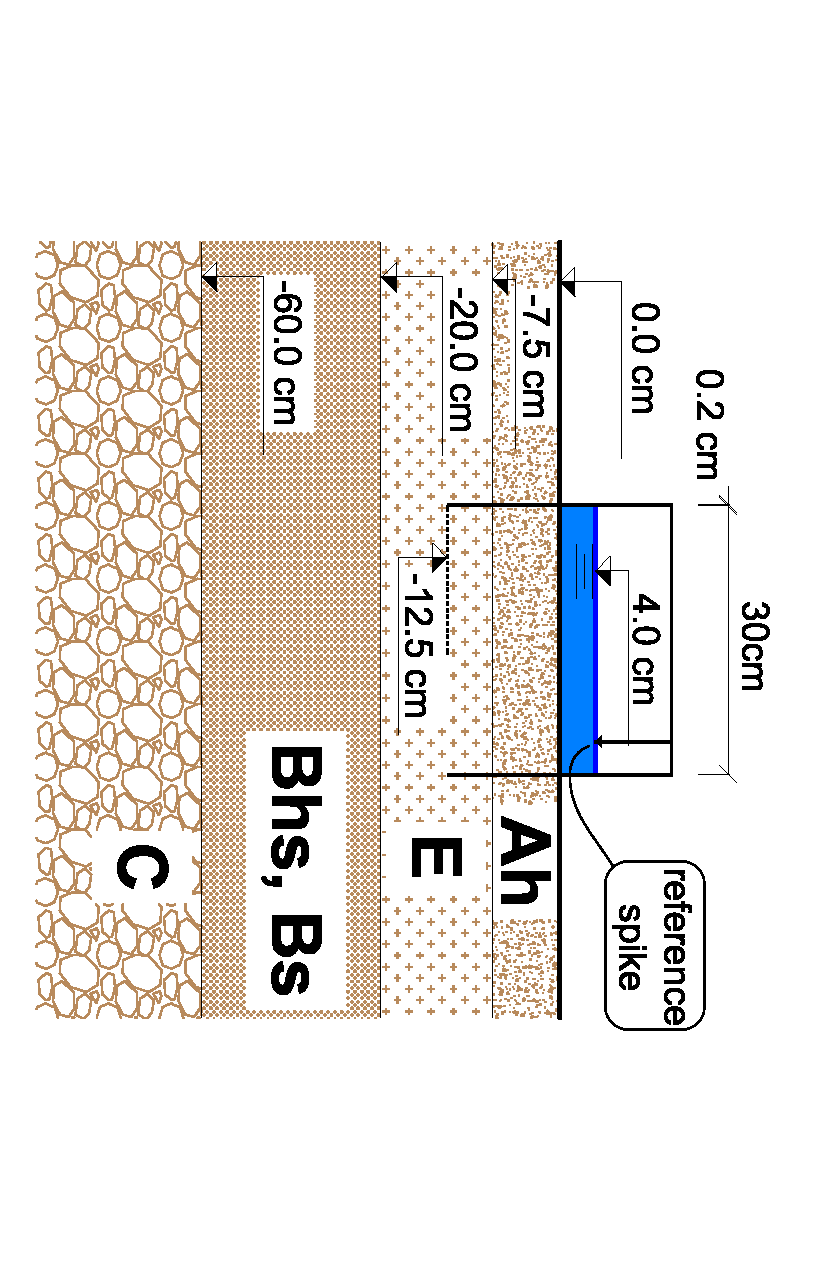
\includegraphics[height=7.5cm]{valec-exp.pdf}}
 \caption{Scheme of the single ring infiltration experiment and the soil layers. }
 \label{experiment}
\end{figure}

The single ring infiltration method (SR) for identifying the soil hydraulic parameters (SHP) of the Ah and E horizons was used here. 
For the Ah horizon, the smoothed experimental data for unsteady SR infiltration were used as the input for inverse modeling of the Richards equation, where the entire parameter set, as given in section~\ref{shp}, was identified. For the E horizon, the experimental data of the steady state part of the SR infiltration were evaluated in a standard way in order to obtain the saturated hydraulic conductivity of this lower layer.  
Details of these experiments have already been published in~\citep{Jacka1}. In brief, the experimental setup was as follows. A steel ring 30~cm in inner diameter, 25~cm in length, and 2~mm in thickness was inserted into the soil to a depth of 12.5~cm, see figure~\ref{experiment}. The interior surface of the ring was flooded to a mean depth of 4~cm. The depth of ponding was kept approximately at a constant level defined by a reference spike, which was placed 4~cm above the surface of the soil. After the water level dropped below the reference spike, a known volume was refilled into the infiltration ring, and the time was logged. The experiment continued until a
quasi-steady infiltration rate ($i_c$) was reached. This took between 40~minutes to 2~hours. An average experiment duration was 60~minutes.

Guelph permeameter measurement (GP) was used for estimating the saturated hydraulic conductivity of the lower horizons. When evaluating horizon E, the measurements were performed in wells ranging in depth between 19~cm  and 26~cm. For the spodic horizon the depth of the measurement wells ranged between 30~cm  and 56~cm. The constant head GP method applied here is described in~\citep{Jacka1}.

\subsubsection{Processing the experimental data from single ring infiltration}
\label{krivka}

A total of 22 SR experiments were conducted on the site. Statistical description of these infiltration data is given by~\citep{jacka-site}, see datasets collected on site 3. The experiments were evaluated as follows. In order to eliminate noise from the experimental values, each SR experiment data set was smoothed. It was observed that the Schwarzendruber analytical model of one-dimensional infiltration exhibited an excellent fitting quality, with the mean  Nash-Sutcliffe model efficiency coefficient value estimated as 0.9974. So we made use of  exponential data smoothing here. The Schwarzendruber equation for cumulative infiltration  states that
\begin{lineq}
I(t)=\frac{\bar{S}\left(1-\exp\left(-A_0\sqrt{t}\right)\right)}{A_0}+\bar{K}_{s}t,
\label{vyhlaz}
\end{lineq}
where $I$ is the cumulative infiltration [$L$], and where the parameter set $A_0$, $\bar{S}$, $\bar{K}_{s}$ is usually expressed in terms of SHPs. This physically based interpretation of the Schwarzendruber parameters is disregarded here, because our infiltration model does not meet the prerequisites for the Schwarzendruber model. The Schwarzendruber model was  considered here as some exponential smoothing function only without any physically  based interpretation.


According to the normality tests,  all three datasets of  parameters $A_0$, $\bar{S}$, $\bar{K}_{s}$ can be well approximated  using a log-normal distribution. The geometric mean is therefore suitable for estimating representative values of these parameters. Representative values are as follows: $\bar{K}_s = 5.16\times 10^{-6}$~m.s$^{-1}$, $\bar{S} = 8.55\times 10^{-4}$~m.s$^{-0.5}$, and $A_0 = 0.1132$~[-]. The evaluated representative  parameter set, together with  model~\eqref{vyhlaz}, will be used as an input curve for identifying the top soil hydraulic parameters (SHP). SHPs of the lower horizons were estimated from direct measurements, as will be described in the next section.




\subsubsection{Obtaining the soil hydraulic parameters of the lower horizons}%[lukas]
\label{dolni}


The average saturated hydraulic conductivity for the E horizon was obtained both from the single ring infiltration experiment (SR) and from the Guelph permeameter measurement (GP). The average hydraulic conductivity for the spodic horizon (Bhs, Bs) and for the weathered bedrock C were evaluated from the Guelph permeameter measurement (GP) only.
As is depicted in figure~\ref{experiment}, the depth of the infiltration ring is below the boundary between Ah (top horizon) and the E horizon. If we assume that the saturated hydraulic conductivity of the top soil horizon is higher than the saturated hydraulic conductivity of the E horizon, then the steady state infiltration rate could be used for estimating this parameter.



A total of 22 SR experiments (as mentioned in section~\ref{krivka}) and 28 GP experiments were conducted to estimate the saturated hydraulic conductivity of the E horizon. The estimated saturated hydraulic conductivity obtained from the SR measurements for this horizon and for the study site does not differ significantly from the saturated hydraulic conductivity originating from the GP experiments (see the results published in \citep{Jacka1}).
 The representative saturated hydraulic conductivity for the E horizon was evaluated as 4.0$\times 10^{-6}$~m.s$^{-1}$.


In total 19 GP experiments were conducted to estimate the saturated hydraulic conductivity of the spodic horizon. The estimated geometric mean value is: $K_s =  1.5\times 10^{-6}$~m.s$^{-1}$.

The saturated hydraulic conductivity of the weathered
    bedrock C was obtained as the geometric mean  from 8 experiments performed using the GP method  in wells from 68 to 130 cm in depth. The estimated mean geometric value is: $K_s =  8.5\times 10^{-6}$~m.s$^{-1}$.

%%%%%%%dat za lukasovi rovnice.
Representative parameters of the retention curves (for the eluvial horizon below the top-soil, spodic horizons and weathered bedrock) were estimated using the soil texture and the bulk density information and a neural network prediction (a type of pedo-transfer function) of Rosetta code, see \citep{Schaap}. 

It is well known that pedotransfer functions work well for spodic and eluvial horizons characterized by high percentage of sand, without a distinct structure, and with a bulk density and porosity corresponding to a standard mineral soil. And thus parameters representing the retention curves for spodic horizons and eluvial horizon below the top-soil were estimated using the soil texture and the bulk density information with pedotransfer function implemented in Rosetta code~\citep{Schaap}.
%%%%%%%%%

The estimated soil hydraulic parameters (SHP) for the lower horizons below the top soil are depicted in table~\ref{tab_SHP}.

\begin{table}[ht]
\begin{center}
\caption{Soil hydraulic parameters for the lower horizons.}
\begin{small}
\doublespacing
\begin{tabular}{c c c c c c}
\toprule
Ranges of depths, horizon(s)&\multicolumn{4}{c}{SHPs}\\ \cline{2-6}
[cm]&$\theta_s$ [-] & $\alpha$ [m$^{-1}$]& $n$ [-]& $K_s$ [ms$^{-1}$] & $S_s$ [m$^{-1}$] \\ \hline
% 0 - 7.5, top-soil (O nad Ah)&*from 0.6 to 0.9&*from 2 to 5&*from 1.05 to 1.9&*from 5$\times 10^{-7}$ to 1$\times 10^{-4}$\\
7.5 - 20, eluvial E&0.46&4.65&1.7408&4.0$\times 10^{-6}$ & 0\\
20 - 60 spodic Bhs and Bs&0.47&2.21&1.4494&1.5$\times 10^{-6}$ & 0\\
$>$ 60 weathered bedrock C & 0.50 & 3.52 & 4.03 &  $8.5\times 10^{-6}$ & 0 \\
\toprule
\end{tabular}
\end{small}
\label{tab_SHP}
\end{center}
\end{table}


\subsection{Inverse modeling procedures}
\label{invproc}

\subsection{Mathematical model of the field infiltration experiment -- governing equation}%[michal]
\label{goveq}


The field infiltration experiment is characterized by variably saturated conditions ranging between unsaturated and saturated states. The geometry of the flow is inherently three-dimensional, but the domain dimension can be reduced by considering the axisymmetric geometry. It is well known that the flux in porous media under variably saturated conditions can be expressed by the Darcy-Buckingham law~\citep{buckingham} \begin{lineq}\label{darcybuck}\vec{q} = -\mathbf{K}(\theta) \nabla H,\end{lineq} where $\vec{q}$ is the volumetric flux [$L.T^{-1}$], $H$ is the total hydraulic head [$L$] defined as $H=h+z$, where $h$ is the pressure head [$L$], $z$ is the potential head [$L$], $\theta$ is the water content [-], and $\mathbf{K}(\theta)$ is the unsaturated hydraulic conductivity  [$L.T^{-1}$]; in general it is a  second order tensor. The relation $\theta(h)$ is referred to as the retention curve, see e.g.~\citep{vangenuchten}.

The law of mass conservation  for incompressible flow in cylindric coordinates  is expressed as (see e.g.~\citep{bear1979})
\begin{lineq}
\label{conti}
-\frac{\partial V}{\partial t} = \frac{\partial q_r}{\partial r} + \frac{q_r}{r} + \frac{\partial q_{\alpha}}{\partial \alpha} + \frac{\partial q_z}{\partial z} ,
\end{lineq}
where $V$ is the volume function [-],  $r$ is the radial coordinate, $\alpha$ is the angular coordinate,  $z$ is the vertical coordinate, and $q_{r, \alpha, z}$ is the  volume flux [$L.T^{-1}$]. The ring infiltration experiment is characterized by rotational symmetric flow, so the angular derivative vanishes. Then the governing equation for  variably saturated and rotational symmetric flow is obtained by substituting the flux in \eqref{conti} by the Darcy-Buckingham law~\eqref{darcybuck}. Together with the consideration of linear elasticity for a porous medium the variably saturated axisymmetric flow in isotropic media is governed by
\begin{lineq}
\label{richaxi}
\left(\frac{\dd \theta}{\dd h} + S_s\frac{\theta(h)}{\theta_s} \right) \frac{\partial h}{\partial t}  =  \frac{\partial K(h) \frac{\partial H}{\partial z}}{\partial z} + \frac{\partial K(h) \frac{\partial H}{\partial r}}{\partial r} + c(x)\frac{\partial H}{\partial r},
\end{lineq}
where $S_s$ is the specific storage [$L^{-1}$], $\theta_s$ is the saturated water content [-], and $c(x)$ is the coefificient of the convection for $r$ coordinate [$T^{-1}$], which has to be further explained.

 \begin{figure}
\centering
\rotatebox{90}{
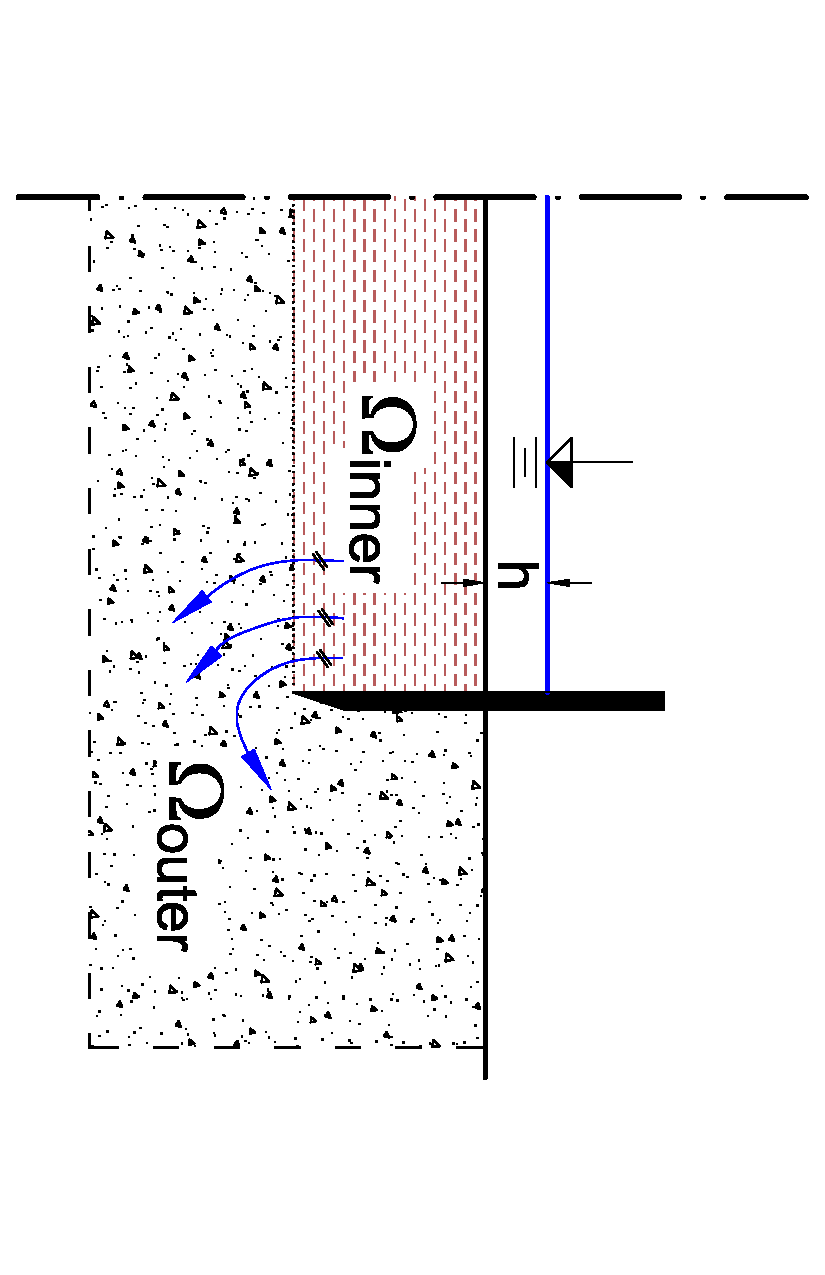
\includegraphics[height=7.5cm]{valcovazk.pdf}}
 \caption{Scheme of the flow domain and the streamlines of infiltration experiment. }
 \label{valecproudy}
\end{figure}

Let us consider the model of the infiltration experiment depicted in figure~\ref{valecproudy}. Let the entire flow domain $\Omega=\Omega_{inner} \cup \Omega_{outer}$, where $\Omega_{outer}$ is the flow domain outside the infiltration ring and $\Omega_{inner}$ is the flow domain within the infiltration ring, exactly as depicted in figure~\ref{valec}. It is apparent that the streamlines inside subdomain $\Omega_{inner}$ are parallel, but the streamlines outside the infiltration ring (inside $\Omega_{outer}$) are axisymmetric.  Then the convection coefficient $c(x)$ is defined as follows
\begin{lineq}
\label{convect}
c(x) = \begin{cases}
	     0 , \quad &\forall x \in \Omega_{inner} \\
	     \frac{1}{r}K(h)\frac{\partial H}{\partial r} , \quad &\forall x \in \Omega_{outer}.
	    \end{cases}
\end{lineq}
Note that $\frac{\partial H}{\partial r} = \frac{\partial h}{\partial r}$, and note that  the flow boundary should not be coincident with the axis of rotation symmetry ($r>0$). Using the standard finite element method approximation, $r$ should even be sufficiently greater than zero (depending on your mesh discretization) to prevent convective dominance. The constitutive relation $\theta(h)$ was substituted by the van Genuchten law~\citep{vangenuchten}, and the constitutive relation $K(h)$ was supplied by the Mualem law~\citep{mualem}.





\subsubsection{Domain scheme, initial conditions and boundary conditions}%[michal]
\label{bccond}
 \begin{figure}
\centering
\rotatebox{90}{
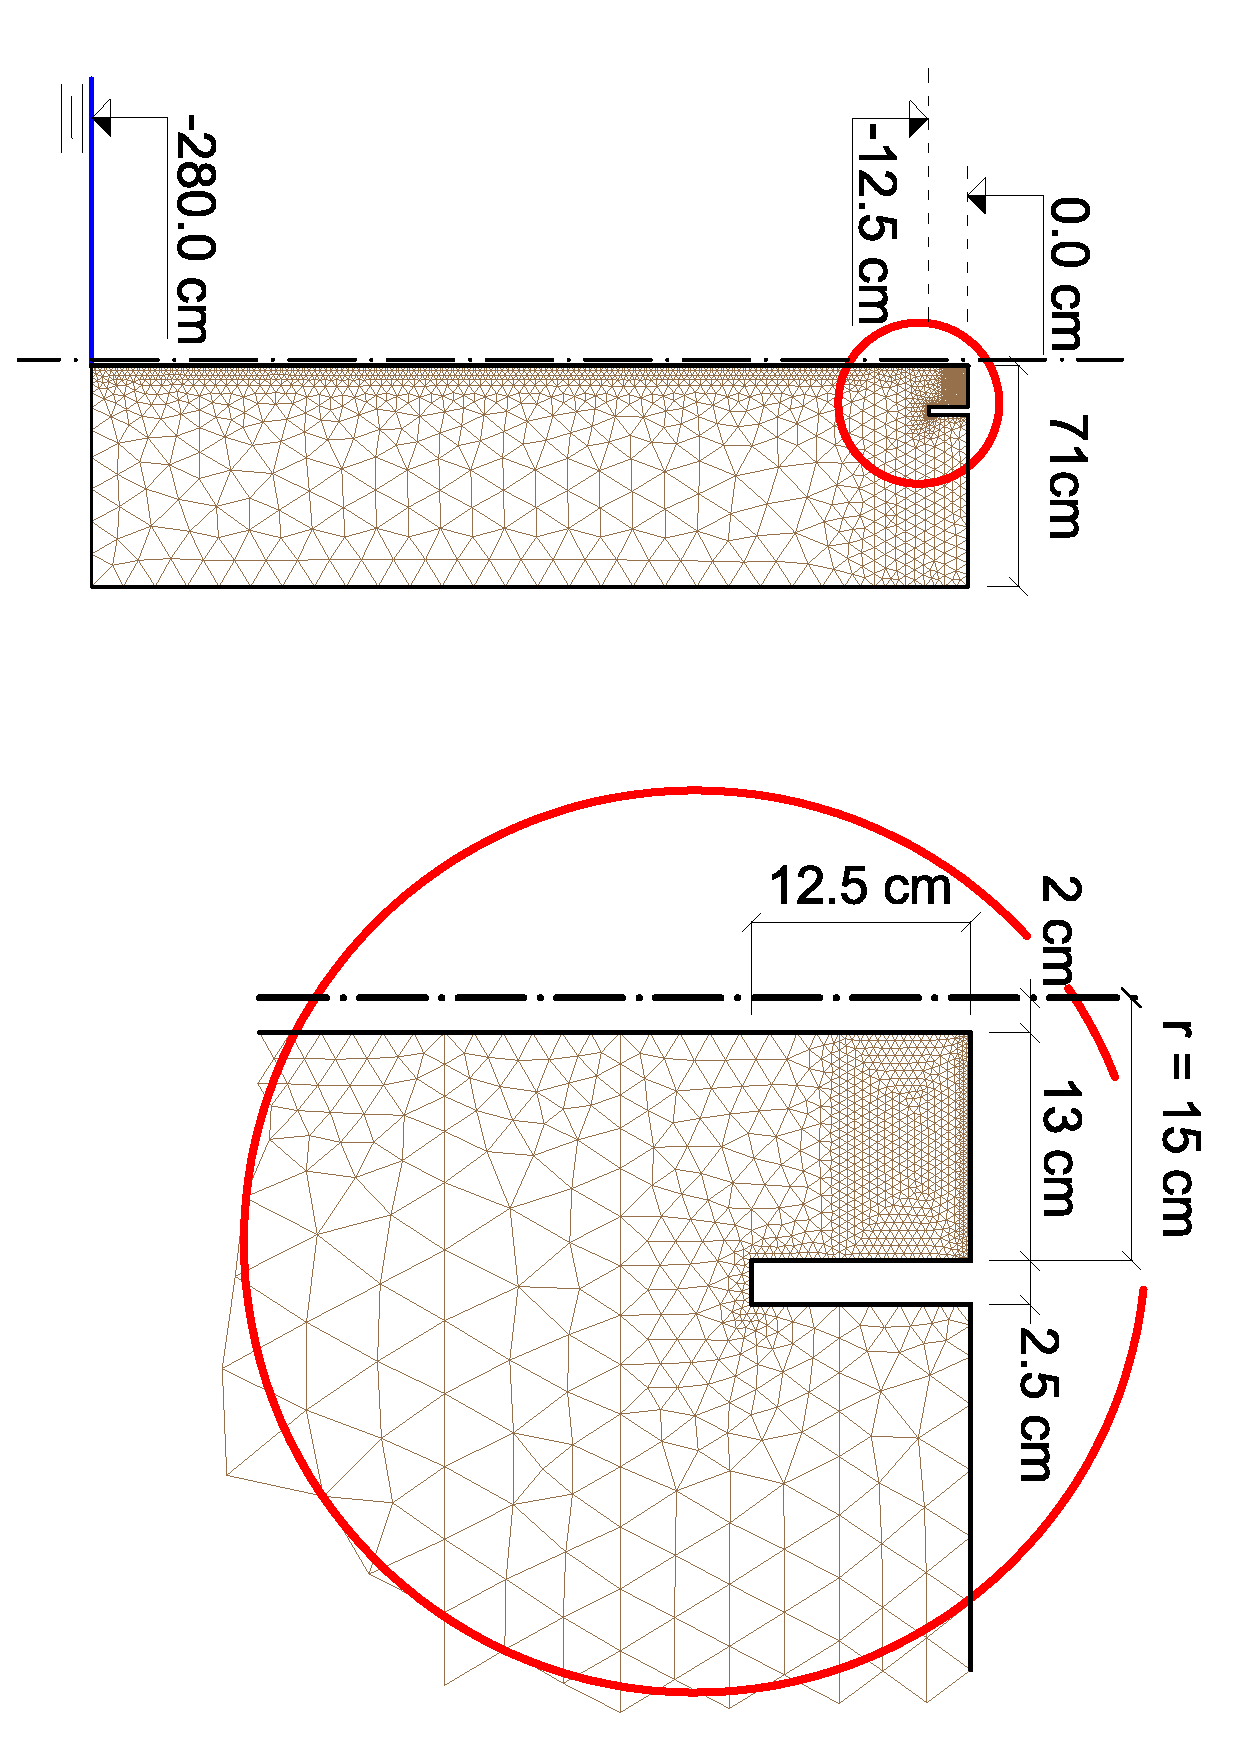
\includegraphics[height=11cm]{infilsit.pdf}}
 \caption{Scheme of the computational domain geometry and domain triangularization.}
 \label{valec}
\end{figure}

The goal of the model was to achieve cumulative infiltration -- the cumulative flux over the top Dirichlet boundary.
The computational domain is depicted in figure~\ref{valec} together with the discretization mesh. The location of the top boundary was natural -- it is the ground surface (inside the ring, it is the Dirichlet condition defining the ponding depth; outside the infiltration ring it is the Neumann condition -- the no-flow boundary). But locating the bottom boundary was more problematic. The following options are available
\begin{itemize}
\item the no-flow boundary (Neumann)
\item the free drainage boundary (Neumann)
\item the groundwater level - zero pressure head (Dirichlet)
\end{itemize}
It is apparent that the wetting front originating from our infiltration experiment affects the soil column only to a certain depth. Defining the Neumann no-flow boundary at a sufficient depth would therefore probably not have a significant effect on the derivative of the solution of \eqref{richaxi} at the top boundary. At the same time, the no-flow boundary is physically incorrect, so this option was rejected. The second option -- the free drainage boundary -- would be completely incorrect here. The free drainage boundary defines fluxes that probably do not appear in our system at all. Above all, if we consider here the initial condition  as a steady state ($\frac{\partial h}{\partial z} = -1$), then the free drainage boundary condition is incompatible with the initial condition, which is again physically incorrect. It turns out that the only physically correct boundary condition for the bottom boundary is the Dirichlet boundary, which represents the groundwater table. The average depth of the groundwater table was known, it is -280~cm below the surface. However, with this particular setup the domain became extremely narrow and deep. However, since the solution at greater depths
is not crucial for estimating the cumulative infiltration we can use coarser  discretization there. Further, if we apply the   adaptive domain decomposition algorithm ($dd$-adaptivity), see~\citep{mojecomp, mojejcam2, mojeamc2},  the non-active parts of the computational domain are sequentially activated and deactivated, and then our current domain extension does not have a significant effect on the computational speed.

%^konec pred obedem

The left hand side domain boundary should be located at a sufficient distance from the axis of anisotropy, because of the term $\frac{1}{r}$ in \eqref{convect}. The Peclet number, representing the numerical stability of convection-diffusion problems is in our case given as follows
\begin{lineq}
Pe = \frac{\frac{\partial h}{\partial r} \Delta x}{2r},
\end{lineq}
where $\Delta x$ is the discretization length [$L$]. Since our mesh is triangular,  $\Delta x$ can be roughly assumed to be the greatest triangle altitude (since we assume some mesh quality properties). Then a sufficient distance from the axis of anisotropy is such that the Peclet number is sufficiently low. If we want to make our computation free of spurious oscillations, a sufficiently low Peclet number means $Pe\le 1$. Therefore, the distance from the axis of anisotropy is given by the domain discretization step at the left hand side boundary.  The selected discretization step at the left hand side boundary was assumed as $\Delta x=2$~cm. The domain was therefore detached by 2~cm from the axis of anisotropy (assuming that $\frac{\partial h}{\partial r} (r,z) < 1, \; \forall (r,z) \in \Omega_{outer}$).

In order to avoid the non-Lipschitz boundary (or any boundary with a shape that is close to the non-Lipschitz boundary) the infiltration ring thickness was oversized  for 2.5~cm. It is obvious that the real ring thickness is much smaller (in our case 2~mm), but reducing the  thickness of the ring yields possible numerical issues but it is expected that it does not significantly affect the solution at the top Dirichlet boundary.

The right hand side boundary was located at a distance $r=73$~cm, it means 50~cm from the infiltration ring. 

 \begin{figure}
\centering
\rotatebox{90}{
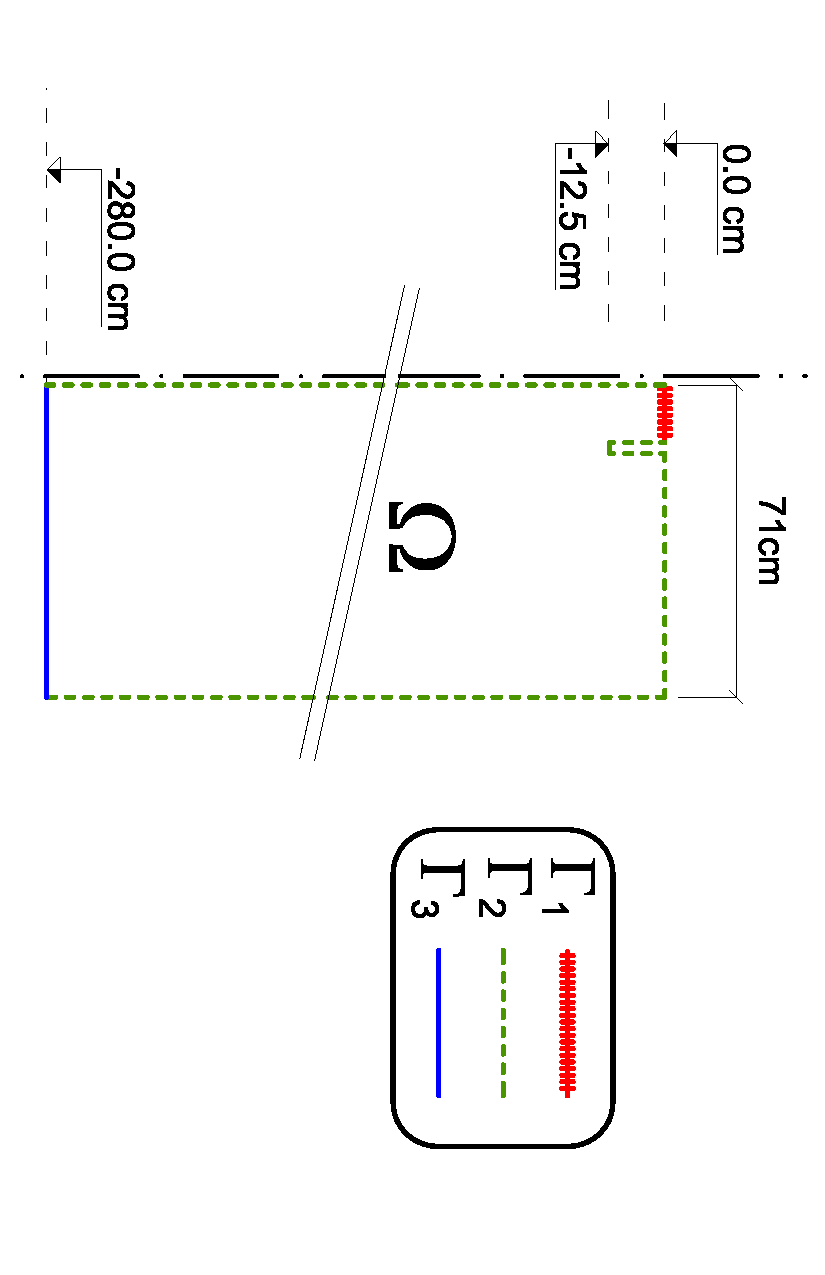
\includegraphics[height=12cm]{schemabc.pdf}}
 \caption{Scheme of the computational domain geometry and the domain boundaries.}
 \label{valecbc}
\end{figure}


The locations of the domain boundaries are depicted in figure~\ref{valecbc}. The boundary conditions are specified as follows
\begin{lineq} 
\begin{split}
h(x,t) &= 4 \; \mbox{cm} \Rightarrow H(x,t) = 4 \; \mbox{cm}; \quad \forall (x,t) \in \Gamma_1 \times [0,T), \\
\frac{\partial H}{\partial \vec{n}} &= 0; \quad \forall (x,t) \in \Gamma_2 \times [0,T), \\
h(x,t) &= 0  \; \mbox{cm}  \; \Rightarrow \; H(x,t) = -280.0  \; \mbox{cm}; \quad \forall (x,t) \in \Gamma_3 \times [0,T).
\end{split}
\end{lineq}
where $T$ is the simulation end time [$T$], and $\vec{n}$ is the boundary normal vector.

The initial condition was assumed as a steady state solution of \eqref{richaxi} before the infiltration experiment. Thus the convection vector $\vec{k}(x) = \left( \begin{smallmatrix} 0 \\ 0 \end{smallmatrix} \right), \; \forall x \in \Omega$, and the boundary condition at boundaries $\Gamma_{1,2}$ was assumed as no-flow boundary. Then the initial condition states that 
\begin{lineq}
H(x) = -280.0 \; \mbox{cm}; \quad \forall x \in \Omega,
\end{lineq}
and thus $\frac{\partial h}{\partial z} = -1$.


\subsubsection{Numerical solution, temporal and spatial discretization, automatic calibration methodology}%[michal]
\label{trapoty}

Equation~\eqref{richaxi} was implemented into DRUtES library~\citep{drutes, mojeamc}. This is an object-oriented library written in Fortran 2003/2008 standard for solving nonlinear coupled convection-diffusion-reaction type problems. The problem was approximated by the linear finite element method for spatial derivatives and Rothe's method for temporal derivatives. The nonlinear operator was treated with the Schwarz-Picard method -- an adaptive domain decomposition  ($dd$-adaptivity) -- with the ability to activate and deactivate subregions of the computational domain sequentially, see works~\citep{mojecomp, mojejcam2, mojeamc2}).



 The domain was nonuniformly discretized by a triangular mesh. The smallest spatial step was considered for the top layers inside the infiltration ring, close to the Dirichlet boundary. The mesh is depicted on figure~\ref{valec}. The minimal spatial step was 0.5~cm, and the maximal spatial step was 20~cm. The domain was discretized with 2097 nodes and 3861 elements. The coarse mesh for the $dd$-adaptivity method was a uniform quadrilateral mesh with elements 17.75$\times$28.0~cm, i.e. a total of 40 coarse elements and 55 nodes. The purpose of the coarse mesh is to organize the elements of the domain triangularization into a so-called clusters, which form a basic unit for the adaptive domain decomposition used here for solving the nonlinear problem, details can be found in~\citep{mojeamc2}.

 
 The spatial and temporal discretization of \eqref{richaxi} leads into sequential solutions of systems of non-linear equations, see e.g.~\citep{mojecomp}. The system was linearized, as discussed in~\citep{mojejcam2, mojeamc2}, and so the numerical solution requires an iterative solution of 
\begin{lineq}
\label{matice}
\mathbf{A}(\vec{x}_l^k) \vec{x}_l^{k+1} = \vec{b}(\vec{x}_l^k),
\end{lineq}
where $k$ denotes the iteration level, and $l$ denotes the time level, until \begin{lineq} \label{picard} ||\vec{x}_l^{k+1} - \vec{x}_l^k||_2 < \varepsilon , \end{lineq} where $\varepsilon$ is the desired iteration criterion.

If the nonlinear problem is treated as 
\begin{lineq}
\label{matice2}
\mathbf{A}(\vec{x}_{l-1}) \vec{x}_l = \vec{b}(\vec{x}_{l-1}),
\end{lineq}
 we have introduced a kind of semiexplicit approximation  
of~\eqref{richaxi}. It is apparent that for short time stepping the method converges to the exact solution. But for the inappropriate time stepping, the method is less accurate, but is also free of possible issues related to the convergence of the nonlinear operator.

Since the infiltration flux is obtained from the numerical derivative of the solution of \eqref{richaxi},  and since it is well known that inaccurate approximation of the capacity term (time derivative term) yields inaccurate mass properties~\citep{celia}, we are aware of a possible impact of spatial and temporal discretization on the identified SHP values. But we are also aware of possible difficulties with convergence of the linearized discrete system~\eqref{matice} for certain combinations of SHPs values within the ranges given in table~\ref{rozsahy} during the automatic calibration, as discussed in~\cite{beven2003-uncertain}.
And thus the following methodology for the automatic calibration was proposed here.

\begin{enumerate}
\item Proceed the calibration procedure with the quasi-explicit stable numerical technique for treating the nonlinear operator explained in equation~\eqref{matice2}, with the initial time step $t_{init}= 10^{-6}$~hrs, and for each subsequent time level $l$, $\Delta t_l = 1.05 \Delta t_{l-1}$, where $l=\{1,n_t\}$, where $n_t$ is the number of time levels used for the temporal discretization; the $dd$-adaptivity algorithm wasn't used at this step. The ranges of parameters for this calibration are given in table~\ref{rozsahy}, so the maximal values of SHP are defined as a vector $\vec{p}^{r_f}_{max}$, and the minimal values are defined as a vector $\vec{p}^{r_f}_{min}$. The spatial discretization for this step of calibration was given in the beginning of this section -- 2097 nodes and 3861 elements. 
Let us assume that this discretization is given by a mesh density function ${\Delta}(\vec{x})^{r_f}$. The function $\Delta(\vec{x})^{r_f}$ is understood as a spatial distribution of mesh size density, which was used as an input for the mesh generator~\citep{t3d}. The superscript $r_f$ defines the refinement level, where $r_f=0$ at this particular stage, and the vector $\vec{x}$ refers to spatial coordinates inside the domain $\Omega$.
\item Let us pressume that this inverse model will have more than just a single solution, this is an assumption of multimodality, which is based on~\citep{beven2003-uncertain}. \begin{itemize} \item Then this calibration will generate vectors of SHPs values $\vec{p}^{i_e}_{r_f}$, where the superscript $i_e$ denotes the number of some  particular local extreme. \end{itemize} 
\item To validate the inverse modeling results, select physically acceptable local extremes and create a scatter plot of the objective function in its neighborhood  with improved temporal integration and spatial discretization. Increase the discretization level $r_f=r_f+1.$ Then 


 Use Schwarz-Picard method for solving the nonlinear system~\eqref{matice}. The iteration criterion for the Picard method was considered as $\bar{\varepsilon}^{r_f}= 10^{-3}$~cm. Again the super script $rf$ denotes the number of the Picard criterion refinements, which is is still $r_f=0$. Initial time step was $t_{init} =  10^{-8}$~hrs. Time step adaptivity was given by the Retention curve zone approach, see~\citep{mojeamc}. Combine the improved numerical scheme for temporal integration with the refined mesh, where ${\Delta}(\vec{x})^{r_f+1}$ and make the scatter plot again. \label{ll0}
  \begin{enumerate}
    \item \label{ll1} If the scatter plots for selected numerical method differ a lot proceed the calibration  again, with the new parameter range defined as $\vec{p}_{max} = 1.1\vec{p}_{r_f}$ and  $\vec{p}_{min} = 0.9\vec{p}_{r_f}$. Let us assume that this calibration will generate a vector of SHPs values $\vec{p}_{t}$.
    \item \label{ll2} Perform the validation again with Picard iteration criterion $\varepsilon^{rf+1}=0.1\varepsilon^{rf}$, and with the refined spatial mesh (use one half of the previous spatial step size).
    \item Create scatter plots again and validate them again with further refinements as discussed in~\ref{ll0} with the refined parameters of the numerical approximation as given in~\ref{ll2}, and if needed return to the step~\ref{ll1} with the increased refinement level $rf=rf+1$.
    \item If there is no further refinement needed exit the calibration process.
  \end{enumerate}
\end{enumerate}


The following sections will further explain the definition of the objective function and the parameter identification algorithm.



\subsection{Parameter identification, a definition of the objective function} %[michal]
\label{objdef}

The soil hydraulic parameters (SHP) of the top soil that will be identified were specified in section~\ref{shp}.
Since the parameters will be identified using a stochastic method, we have to introduce a physically reasonable range for each parameter. The ranges for the SHPs are specified in table~\ref{rozsahy}.

\begin{table}[ht]
\begin{center}
\caption{Ranges of SHPs ($\vec{p}_{max}$ and $\vec{p}_{min}$ for identifying the SHPs in the top-soil layer.}
\begin{small}
\doublespacing
\begin{tabular}{c c c c c}
\toprule
% Ranges of depths, horizon(s)&\multicolumn{4}{c}{Input values for inverse modelling}\\ \cline{2-5}
$\theta_s$ [-]&$\alpha$ [m$^{-1}$]&n [-]& $K_s$ [m.s$^{-1}$] & $S_s$ [m$^-1$] \\ \hline
\toprule
0.25 -- 0.90 & 0.01 -- 5.0 & 1.05 -- 2.10 & $10^{-7}$ -- $10^{-4}$ & 0.0 -- 10.0 \\
\toprule
\end{tabular}
\end{small}
\label{rozsahy}
\end{center}
\end{table}

The objective function is defined in the following paragraph.


Let $\bar{I}(\vec{p},t)$ be the cumulative infiltration obtained from solving the mathematical model~\eqref{richaxi} bounded by the initial and boundary conditions  defined in section~\ref{bccond} for a certain vector of SHP $\vec{p}$ considered as
\begin{lineq}\bar{I}(\vec{p},t) = \frac{\int\limits_0^t \int\limits_{\Gamma_1}-K \frac{\partial H}{\partial \vec{n}}(t)  \dd \Gamma_1 \dd t}{\int\limits_{\Gamma_1} \dd \Gamma_1}.\end{lineq}
Let $I(t)$ be the cumulative infiltration defined by \eqref{vyhlaz} with parameters given in section~\ref{krivka}. 
Then the objective function was defined for three different criteria in order to avoid ill-posed objective function definition.

The objective functions were defined as follows:
\begin{enumerate}
\item the first criterion $\Psi_1$ was defined as $L_2$ norm of the difference between the  experimental and model data and thus
\begin{lineq}
\label{objektiva1}
\Psi_1 (\vec{p}) = \sqrt{\int\limits_0^{T_{end}} \left( \bar{I}(\vec{p},t) - I(t) \right)^2 \dd t},
\end{lineq}
where $T_{end}$ is the final simulation time [$T$],
\item the second criterion was the $L_{\infty}$ norm of the difference between the experimental and model data and thus
\begin{lineq}
\label{objektiva2}
\Psi_2 (\vec{p}) = \mathrm{sup} \left( \sqrt{\left( \bar{I}(\vec{p},t) - I(t) \right)^2} \right), \quad  t \in (0, T_{end}),
\end{lineq}
\item and the third criterion was considered as the difference between the final derivatives between the model data and the experimental data
\begin{lineq}
\label{objektiva3}
\Psi_3 (\vec{p}) =  \sqrt{\left( \frac{\dd \bar{I}(\vec{p},T_{end})}{\dd t} - \frac{\dd I(T_{end})}{\dd t} \right)^2}.
\end{lineq}
\end{enumerate}
And so we have applied here a multi-objective optimization.



\subsubsection{Optimization method}%[matej]
\label{optima}

The most traditional way of dealing of multiple objectives in optimization is the Weighted Sum Method (WSF). Each objective out of $kk$ objectives $f_i(\vec{x})$ is multiplied by user defined weights $w_i$ and their sum is optimized. The problem is converted into single criteria optimization:
%
\begin{lineq}\label{MO}
    F(\vec{x}) = \sum_{i=1}^{kk} w_i f_i(\vec{x}) , \quad\quad \sum_{i=1}^{kk} w_i = 1, \quad w_i \ge 0 ,
\end{lineq}
and any single-objective optimization method can be used to solve~\eqref{MO}. Although this method is really easy and intuitive, the biggest obstacle is in setting the weights. The weights express the relative importance of individual objectives, which, in real world applications, is difficult to determine. The success of the WSM depends also on scaling of objectives; all of them should have more or less the same order of magnitude to affect the value of $F(\vec{x})$ similarly. Therefore, not only weight vector must be set, but also a~normalization of objectives must be performed. Similarly to weight vector, it is difficult to determine in advance which objectives' values can be reached and accordingly, to properly set the normalization vector.

It seems to be advantageous to use population-based Evolutionary Algorithms to obtain the Pareto set for general multi-objective optimization problem.

In this contribution, a genetic algorithm called GRADE \citep{grade,Kucerova:2007:PHD} was applied. It is a real-coded genetic algorithm combining the ideas of genetic operators: cross-over, mutation and selection taken from the
standard genetic algorithm and the idea of differential operator taken from the differential evolution.
Moreover, the algorithm GRADE is supported with the niching method
CERAF, which was developed based on an idea of enhancing the algorithm with
memory and restarts~\citep{ceraf}. When the GRADE algorithm loses the convergence, the current position of the optimization algorithm is marked as a local extreme and a forbidden area is build around in order to forbid the optimization algorithm again to fall into the same local extreme. Hence all inspected local extremes are stored in memory and can be inspected after the optimization. 

The main setting of the optimization procedure was as follows: the population of the genetic algorithm contains 30 independent solutions, the whole identification stops after 20.000 objective function evaluations and a local extreme was marker after 600 evaluations without any improvement.


\section{Results and discussion} %[michal, lukas]
The first step in parameter identification should always be the sensitivity analyses in order to evaluate the sensitivity of the given objective functions~\eqref{objektiva1} -- \eqref{objektiva3} for the searched parameter set. The sensitivity analyses was conducted for the given SHPs ranges (see table \ref{rozsahy}). In total 10.000 samples of the objective function \eqref{objektiva1} ($L_2$ norm of the model error) were evaluated, in order to obtain the  Total Sobol Index for each parameter, see e.g.~\citep{kniha-citlivost}. The values of the Total Sobol Indices are given in table~\ref{citlivost}. Since the evaluated Total Sobol Index for each parameter was nearly 0.9, our model exhibits an excellent sensitivity for all SHPs parameters.

\begin{table}[ht]
\begin{center}
\caption{Total Sobol indices for the searched SHPs parameters.}
\begin{small}
\doublespacing
\begin{tabular}{l||c c c c c}
\toprule
% Ranges of depths, horizon(s)&\multicolumn{4}{c}{Input values for inverse modelling}\\ \cline{2-5}
parameter & $\alpha$ & $n$ & $K_s$ & $\theta_s$ & $S_s$ \\ \hline
\toprule
Total Sobol Index & 0.850 & 0.921 & 0.876 & 0.868 & 0.884 \\
\toprule
\end{tabular}
\end{small}
\label{citlivost}
\end{center}
\end{table}

As stated in the section~\ref{trapoty} SHPs parameters were initially searched in the wide intervals defined in table~\ref{rozsahy} with the less accurate numerical technique~\eqref{matice2}. Since the proposed parameter search algorithm handles an ability for identification of  local extremes we could perform a test of multimodality. 
There were in total 33 points on Pareto front identified. The identified Pareto front was non-convex. 
There were in total 8 local extremes  with different fitting qualities identified on the non-convex Pareto front -- see table~\ref{shp-vysledky} for particular SHPs values and the following fitting quality descriptors -- namely the coefficient of determination, the intercept, and the slope, see table~\ref{shp-vysledky}. It is well known, see e.g. \citep{r2andslope}, that only the accoplishable values of the coefficient of determination does not guarantee good fitting qualities.

\begin{table}[ht]
\begin{center}
\caption{Identified local extremes of Pareto front during the first run of parameter search procedure.}
\begin{small}
\doublespacing
\begin{tabular}{l || c c c c c || c c c }
\toprule
no. & $\alpha$ [m$^{-1}$] & $n$ [-] & $\theta_s$ [-] & $K_s$ [m.s$^{-1}$] & $S_s$  [m$^{-1}$] & $R^2$ & intercept & slope\\ \hline \hline
{\bf 1} & \num{2.447e-2} &  2.45 & 0.25 & \num{.00000006944444444444} & 0.419  & 0.9914  & 1.9395 & 0.6891  \\ \hline
{\bf 2} & 0.101 & 1.6517 &  0.271 & \num{.00000303333333333333} &  \num{2.879e-2} & 0.9989 & -0.6895 & 0.9861 \\ \hline
{\bf 3} & \num{1.840e-2} & 2.098 & 0.353 & \num{.00000361666666666666} & \num{1.845e-2} & 0.9955 & 1.9215 & 0.9278 \\ \hline
{\bf 4} & 0.157 & 1.968 & 0.720 & \num{.00000557407407407407} & \num{1.053e-3} & 0.9966 & 0.9539 & 0.9607 \\ \hline
{\bf 5} & 0.150 & 1.586 & 0.720 &  \num{.00000303611111111111} &  \num{7.641e-3} & 0.9985 & 0.0025 & 0.9973 \\ \hline
{\bf 6} & 0.258 & 2.152  & 0.401 &  \num{.00000304250000000000} & 0 & 0.9980 & -0.0320 & 0.9958 \\ \hline
{\bf 7} & 0.380 & 1.279 & 0.594 &  \num{.00000323333333333333} & 0 & 0.9996 & 0.2000 & 0.9884 \\ \hline
{\bf 8} & 0.255 & 1.384 & 0.254 &  \num{.00000310833333333333} &  \num{1.922e-2} & 0.9995 & 0.1520 & 0.9919 \\
\toprule
\end{tabular}
\end{small}
\label{shp-vysledky}
\end{center}
\end{table}

The local extremes 5-8 have acceptable fitting qualities -- see figure~\ref{obrazky}, however the identified retention curve parameters are highly distuingshed -- see figure~\ref{ret-krivky}.

Apart the local extreme no. 1 all solutions have more or less good fitting qualities, and the local extremes 5,6,7,8 have even excellent fitting qualities.  As given in table~\ref{shp-vysledky} we are able to assign to our infiltration experiment different porous media with distinguished properties -- especially the saturated water content $\theta_s$ -- exactly as expected in~\cite{beven2003-uncertain}. This non-uniqueness in our inverse analyses can be resolved by selecting the local extremes with physically appropriate SHPs values. The highlighted local extreme  no. 7 has physically expectable values of SHPs, and, surprisingly, also the best value of the coefficient of determination. However, the best value of the determination coefficient together with the physically acceptable values of SHPs parameters is rather a coincidence here. The plot of this fit is depicted in  figure~\ref{fits} -- left.

\begin{figure}
  \hfill
  \begin{minipage}[t]{.45\textwidth}
    \begin{center}  
\rotatebox{-90}{
  \includegraphics[height=7.cm]{good-fit.eps}}
\end{center}
\end{minipage} 
\begin{minipage}[t]{.45\textwidth}
 \begin{center} 
\rotatebox{-90}{
\includegraphics[height=7.cm]{bad-fit.eps}}
\end{center}
\end{minipage}
\caption{Left: The best model fit obtained for the less precise numerical treatment -- \eqref{matice2}, $R^2= 0.9994$, local extrem no. 7, Right: Model validation for the improved numerical treatment -- \eqref{matice}, $R^2= 0.9869$. }
\label{fits}       % Give a unique label
\end{figure}

In the next stage the previously identified SHPs set for the local extreme no. 7  was validated with the improved treatment of the nonlinear operator -- see equation~\eqref{matice}. The nonlinear system was linearized by simple Picard method, the stopping criterion $\varepsilon$ (see~\eqref{picard}) was equal to 10$^{-4}$~cm. As expected the improved numerical treatment affected the previously identified solution and the reevaluated coefficient of determination was $R^2=0.9869$. The plot of this solution is depicted in figure~\ref{fits} -- right.

Despite the fact the validated model fit still preserved reasonable fitting qualities, the inverse analyses was re-evaluated for SHPs ranges given in step 3. The updated SHP parameter set states as follows
\begin{itemize}
\item  $\alpha= 0.329$~m$^{-1}$, $n=$            1.31385 [-],  $\theta_s=$  0.593 [-], $S_s$ = 0.0~m$^{-1}$, $K_s$ = \num{.00000304622222222222}~m.s$^{-1}$.
\end{itemize}
The updated coefficient of determination was $R^2=0.9985$. In order to eliminate the effect of spatial discretization, the model with a proper non-linear operator treatment was validated with refined spatial discretization -- exactly as defined in stage no. 4 in the calibration methodology. The finally updated coefficient of determination did not significantly differed from the previous one, and thus the original spatial discretization was probably accurate enough for our inverse analyses.

The updated SHPs parameter set with the proper non-linear operator strategy  -- \eqref{matice} (calibration methodology no. 3)  did not significantly differ from the SHPs obtained with the less precise nonlinear operator treatment -- \eqref{matice2}. And thus this simple but  stable treatment  of the Richards equation operator provided a good estimate for the searched SHPs parameter set.

\section{Conclusions} %[michal, lukas]

This paper has presented an evaluation of the soil hydraulic parameters (SHP) of a mountainous podzolic soil profile. The SHP values for the lower horizons were identified on the basis of standard methods -- a single ring (SR) infiltration experiment and a Guelph permeameter (GP). The SHPs values for the top soil layer were identified on the basis of an inverse analysis of the development of the SR experiment in time. The main objective of this paper was to present an inverse analysis of the topsoil layer.  Since the SR experiment is an inherently three-dimensional process, where the streamlines within the infiltration ring are parallel, but outside the infiltration ring the streamlines are rather axisymmetric. The governing equation for the mathematical concept has been presented here. Since the convective term in the governing equation for axisymmetric flow incorporates the inverse of the distance from the center of the axisymmetric coordinates, which is the center of the infiltration ring, it was necessary to pay attention to an issue related to convective dominance.

The issue of the initial and boundary condition setup has also been discussed here. It was found  that the only physically correct  initial and boundary conditions setup for our  case requires the groundwater table as the bottom boundary condition, despite the fact that it is apparent that the infiltration process cannot interfere with the soil profile so deep below the surface.  We made use here of the adaptive domain decomposition method ($dd$-adaptivity), which enables the computational domain to be split into active and non-active parts. Thus the selected domain extension did not significantly affect the computational speed -- this method has been developed and implemented into DRUtES opensource project~\citep{drutes}.

The equifinality -- non-uniqueness --  of this Richards equation based inverse model was tested. We have found several solutions with distinguished parameter setup, but with excellent fitting qualities. This observation is not so surprising,  since we can take into consideration, that the experimental data can be well interpreted with three-parametric Schwarzendruber equation, and the Richards equation is four or five parametric equation (depending whether we use non-zero specific storage or not). In order to resolve this non-uniqueness, only the parameter set with the physically appropriate values was selected. Coincidentally, it was also the parameter set with the best value of the coefficient of determination -- the global extreme -- however the local extremes with highly distinguished SHPs values exhibited very similar fitting qualities as the global extreme, so we cannot simply conclude, that global extreme has always the best physical interpretation of the inverse model. It turns out that it is useful to inspect local extremes as well, which is, unfortunately,  often non-trivial.



% Since the numerical solution of the governing equation is strongly affected by discretization in time and space, the parameters were identified on  nine models with different spatial and temporal discretization.
% The minimum of the objective function was searched using a  stochastic method -- differential evolution -- implemented by~\citep{Mullen11} in R~project~\citep{Rstudio}.
% 
% It was observed that the identified  saturated hydraulic conductivity, together with the specific storage, were not so sensitive to different spatial and temporal discretization. However, the parameters of the retention curve $\alpha$ and $n$ were highly sensitive to spatial discretization. The saturated water content exhibited very low correlation with the objective function. The values identified with our stochastic method were more likely just random numbers.  This inverse analysis was therefore completely inappropriate for a search for this parameter. Surprisingly, the saturated hydraulic conductivity of the top-soil layer also exhibited very low sensitivity. However, unlike the saturated water content values, the identified saturated hydraulic conductivity values for all nine experiments were very similar,  and provided a physically reasonable value. 

Finally, it could be concluded, that our model was in a good agreement with the experimental data, and the identified representative soil profile can be used e.g. as an input for a deterministic catchment runoff model.

\section{Acknowledgement}

Financial support from the Czech Science Foundation (research project GACR 13-11977P) is gratefully acknowledged.

% \section*{References}

\bibliography{mybibfile}


\end{document}
